\documentclass{article}
\usepackage{fullpage}
\usepackage{amsthm}
\usepackage{amsmath}
\usepackage{amsfonts}
\usepackage{amssymb}
\usepackage{mathrsfs}

\usepackage{graphicx}

\usepackage[algoruled]{algorithm2e}
\usepackage{listings}
\lstset{language=python}  

\newcommand{\blind}[2]{#1}

\newtheorem{thm}{Theorem}
\newtheorem*{thm*}{Theorem}
\newtheorem{lemma}[thm]{Lemma}
\newtheorem*{lemma*}{Lemma}

\theoremstyle{definition}
\newtheorem{definition}[thm]{Definition}


\begin{document}

\title{Measurement linkage using Markov Link Intervals}

\author{\blind{Jackson Loper$^{a,b}$\footnote{To whom correspondence should be addressed: email jl5116@columbia.edu.}, Trygve Bakken$^c$, Uygar Sumbul$^c$, \\ Gabe Murphy$^c$, Hongkui Zeng$^c$, David Blei$^{b,d}$, Liam Paninski$^{a,b}$ \\
\small $^a$Grossman Center for the Statistics of Mind, Zuckerman Mind-Brain Behavior Institute, \\ \small Department of Neuroscience, and Center for Theoretical Neuroscience, Columbia University, NY NY \\
\small $^b$Department of Statistics, Columbia University, NY NY \\
\small $^c$Allen Institute for Brain Science, Seattle WA \\
\small $^d$Department of Computer Science, Columbia University, NY NY}{[Authors blinded]}}

\maketitle

% https://academic.oup.com/biomet/article/106/1/145/5250868
% We consider nonparametric estimation of a covariance function on the unit square, given a sample of discretely observed fragments of functional data. When each sample path is observed only on a subinterval of length δ<1⁠, one has no statistical information on the unknown covariance outside a δ-band around the diagonal. The problem seems unidentifiable without parametric assumptions, but we show that nonparametric estimation is feasible under suitable smoothness and rank conditions on the unknown covariance. This remains true even when the observations are discrete, and we give precise deterministic conditions on how fine the observation grid needs to be relative to the rank and fragment length for identifiability to hold true. We show that our conditions translate the estimation problem to a low-rank matrix completion problem, construct a nonparametric estimator in this vein, and study its asymptotic properties. We illustrate the numerical performance of our method on real and simulated data.

\begin{abstract}
We consider two datasets, each taking different kinds of measurements from samples of a common population.  The first dataset is constructed by drawing individuals randomly from this population and measuring a quantity about each individual.   The second dataset is constructed similarly, but a different quantity is measured.  ``Unpaired measurement linkage'' attempts to use this data to infer the joint distribution of the two different quantities.  We study this problem in the presence of a third quantity which is observed in both datasets and satisfies a conditional independence assumption.  We characterize identifiability in this case and develop estimators for the joint distribution.  The performance of the estimators is tested in simulations.  The method is applied to transcriptomic measurements to uncover the relationship between two different technologies for measuring gene expression in mouse neurons.
\end{abstract}

\section{Introduction}

Many scientific experiments produce data that come from different measurement techniques.  To use such data, we need to understand the link between the different types of measurements.  For example, in a biological context, a transcriptomic-morphological link would answer a question like:  ``We have measured the transcriptome of this cell -- what might its morphology have been?''

It is particularly challenging to estimate the link when multiple measurements of the same specimen are unavailable.  For example, it is currently often difficult to observe both the RNA expression and morphological properties of a single cell.  Rather, we typically have two datasets: one contains the transcriptomes of one group of cells and the other contains the morphology of another group of cells from the same population.   However, the datasets are not completely disconnected: there is some information which is collected for every specimen in both datasets.  For example, it may be possible to read optogenetic marker information for every cell in both datasets.  The task is to leverage this information to uncover the link.  

This \emph{unpaired measurement linkage} problem arises in many scientific and technological fields where it is difficult to take multiple types of measurements of the same specimen.  Formally, unpaired measurement linkage seeks to estimate a distribution $p(\ell,x,y)$ even though we can never observe a complete sample $(L,X,Y)\sim p$.  For every sample we can observe $(L,X)$ or we can observe $(L,Y)$ -- but we can never observe $(X,Y)$.  In the cell biology example above, $X$ might correspond to a cell's transcriptome, $Y$ might correspond to the cell's morphology, and $L$ might correspond to an optogenetic marker that can be observed for every cell.  

The key challenge in unpaired measurement linkage is to identify good assumptions or inductive biases; without any additional assumptions the problem is always ill-posed.  An overview of different possible assumptions can be found in Fan \emph{et al} \cite{FanYan2017}.  

In this paper, we seek to understand unpaired measurement linkage in the discrete setting under the assumption that $L$ and $Y$ are conditionally independent given $X$.  This assumption is inspired by cell biology, and holds naturally whenever $L$ and $Y$ can be understood as independent noisy measurements of $X$.  For example, in Section \ref{sec:allen} we will see an example where optogenetic markers ($L$) and a low-fidelity transcriptomic record ($Y$) act as independent noisy indicators about cell-type ($X$).  Many other examples can be found in Section \ref{sec:conclusions}.  Note that the side-information $L$ bears a formal similarity to an instrumental variable, but its function is different; instrumental variables resolve causal effects in the presence of unobserved confounders, whereas these variables permit joint inference when only marginal observations are available. 

We investigate the identifiability issues and develop estimators which are asymptotically guaranteed to bound the true joint distribution.  The key idea is to make a detailed study of the ``observational equivalence classes'' \cite{paulino1994identifiability,hauser2012characterization,tong1991indeterminacy}.  Each class corresponds to a set of parameters that give rise to the same distribution on the data we observe.  We show that estimating these sets is actually impossible, but a carefully-chosen dilation of these sets asymptotically contains the true model parameters and also concentrates on the observable distributions.  We also design a simple optimization algorithm to find extremal points in these dilated sets.  These extremal points yield bounds for the parameters which we dub ``Markov Link Intervals,'' because they use the Markov conditional independence assumption to bound the parameter that links $X$ to $Y$.   Finally, we interrogate the effectiveness of these intervals using simulations and real-world data. 

This work arises out of a literature that spans many fields and many decades.  Perhaps the earliest approach to unpaired measurement integration comes from Andrey Kolmogorov, who conjectured an inequality for the cumulative distribution function of the sum of two random variables in terms of their marginal distributions \cite{makarov1982estimates}.  Related inequalities have also been studied in the context of quantum physics \cite{chaves2014inferring}.  More recently, bounds on arbitrary univariate functions $f(X,Y)$ have also been developed in the context of causal inference \cite{balke1994counterfactual}.  Most recently, the CycleGan algorithm has gained prominence in the computer graphics community for successfully estimating a joint distribution between photographs ($X$) and watercolor paintings ($Y$) of the same subject; CycleGan accomplishes this unpaired measurement linkage using two completely separate datasets, one of photographs and one of watercolor paintings \cite{zhu2017unpaired}.  This work connects most directly to the work of Fan \emph{et al} (2017), which gives an extensive study for unpaired measurement linkage problem under many different assumptions \cite{FanYan2017}.  Under each assumption the asymptotics of estimators for $\mathbb{E}[f(X,Y)]$ are characterized, where $f$ can takes a wide variety of forms.  Here we extend this work by considering similar questions under a new kind of assumption.

\newcommand{\DX}{\mathcal{D}^X}
\newcommand{\DY}{\mathcal{D}^Y}
\newcommand{\DV}{\mathcal{D}}
\newcommand{\LL}{\mathcal{L}}
\newcommand{\pr}[1]{\mathrm{pr}\left(#1\right)}

%              _        _   _             
%  _ __   ___ | |_ __ _| |_(_) ___  _ __  
% | '_ \ / _ \| __/ _` | __| |/ _ \| '_ \ 
% | | | | (_) | || (_| | |_| | (_) | | | |
% |_| |_|\___/ \__\__,_|\__|_|\___/|_| |_|
                                        


\section{Markov Link Intervals (MLI)}

Consider a triple of discrete random variables variables, $(L,X,Y) \sim p$. We assume $p$ has support on $\{1\cdots N_L\}\times\{1\cdots N_X\}\times\{1\cdots N_Y\}$ and $L,Y$ are conditionally independent given $X$.  
% We further assume that $N_X > N_L$ (if $N_X\leq N_L$ it is straightforward to show that inference can almost always be performed with ordinary estimation methods).  
We parameterize $p$ as
\[
p(\ell,x,y;\pi,\alpha,\beta)=\pi_\ell \alpha_{\ell,x} \beta_{x,y}
\]
where $\pi$ lies strictly in the interior of the $N_L$-simplex, $\alpha$ is an $N_L \times N_X$ right-stochastic matrix, and $\beta$ is an $N_X \times N_Y$ right-stochastic matrix.  We will also find it useful to let $\gamma_{\ell y}$ denote $p(y|\ell)=\sum_x \alpha_{\ell,x} \beta_{x,y}$. 

Suppose we are given independent samples from $p$, but some data is missing.  Each sample includes $L,X$ or $L,Y$ but no sample ever includes both $X$ and $Y$.  Can we still learn $p$?  Let $n,m>0$ and $(L_1,X_1,Y_1),(L_2,X_2,Y_2) \cdots (L_{n+m},X_{n+m},Y_{n+m})$ denote samples of independent copies of $(L,X,Y)$.  Let
%
\begin{align*}
\DX &= (L_1,X_1),\cdots (L_n,X_n) \\
\DY &= (L_{n+1},Y_{n+1}),\cdots (L_{n+m},Y_{n+m}) 
\end{align*}
%
Unpaired measurement linkage seeks to use the data $(\DX,\DY)$ to estimate the parameters of $p$, namely $(\pi,\alpha,\beta)$.  Observe that estimating $\pi,\alpha$ from this data is straightforward.  

Existing estimation theory is less helpful for the parameter $\beta$.  In this paper we develop theory and practice for estimating $\beta$.

%            _   _                 _   _             
%   ___  ___| |_(_)_ __ ___   __ _| |_(_) ___  _ __  
%  / _ \/ __| __| | '_ ` _ \ / _` | __| |/ _ \| '_ \ 
% |  __/\__ \ |_| | | | | | | (_| | |_| | (_) | | | |
%  \___||___/\__|_|_| |_| |_|\__,_|\__|_|\___/|_| |_|
                                                   


\subsection{Theory}

Correct inferences about $\beta$ require careful treatment of its identifiability.  Our first result is a negative one:

\begin{lemma}[Unidentifiability]  \label{lem:unident} When $N_L<N_X$ there is no generally consistent estimator to infer $\beta$ from the data $(\DX,\DY)$.  
\end{lemma}

Unfortunately, the $N_L<N_X$ regime is precisely the one which motivated our present work, inspired by investigation of cell-types in neuroscience.  This result shows that consistent estimation of $\beta$ may not be possible in our case.

When a parameter cannot be consistently estimated, one common approach is to bound the unidentifiable parameter using  ``observational equivalence classes'' \cite{paulino1994identifiability,hauser2012characterization,tong1991indeterminacy}.  In our case, this equivalence class is defined as the set of all the different parameters $(\pi',\alpha',\beta')$ which would give rise to the true distribution on the observable variables $(\DX,\DY)$.  Even though $\beta$ is unidentifiable, we might hope to identify this set of possible parameters.  Our second result shows this approach is unlikely to succeed:

\begin{lemma}[Discontinuity of observational equivalence classes]  \label{lem:noobseq} Endow the space of observable distributions with the total variation metric.  Endow the space of sets of parameters $\pi,\alpha,\beta$ with the Pompeiu-Hausdorff metric.  The map from possible distributions on $\DX,\DY$ to observational equivalence classes of parameters is not continuous.   This mapping is sometimes discontinuous even around points where the rows of $\alpha$ are linearly independent and all parameters lie in the interior of the natural parameter space.  
\end{lemma}

Even infinitesimal error in the estimation of the observable distribution may thus yield large errors in our estimates of the observational equivalence class.

A partial resolution to this difficulty can be obtained if it is known that $\beta$ is strictly positive and the rows of $\alpha$ are linearly independent.  Under these conditions we can first estimate $\alpha$ and then estimate the observational equivalence class for $\beta$ for the observations $\DY$ under a fixed value for $\alpha$.  It turns out that the distance between this class and $\beta$ does converge to zero:

\begin{thm}[Consistency for positive $\beta$] Let the rows of $\alpha$ be linearly independent and let $\beta_{x,y}\geq c>0$.  Define $\gamma$ as the $N_L\times N_Y$ right-stochastic matrix
\[
\gamma_{\ell y} \triangleq \sum_{x} \alpha_{_\ell x} \beta_{x,y}
\]
Let $\hat \pi, \hat \alpha, \hat \gamma$ denote any consistent estimators for $\pi,\alpha,\gamma$.  Consider $\{\beta':\ \hat \alpha\beta'=\hat \gamma \}$, the equivalence class for the observations $\DY$ after fixing the estimate $\hat \alpha$.  The distance between the point $\beta$ and this set converges to zero in probability.  
\end{thm}

A more general solution can be obtained by seeking a small dilation of the observational equivalence classes.  Let $\LL(\DX,\DY;\hat \pi,\hat \alpha,\hat \beta)$ denote the likelihood of the observed data under the model under the parameters $\hat \pi,\hat \alpha,\hat \beta$.  Let $\LL^*$ denote the maximum value of $\LL$ over all possible parameters.  Define
\begin{gather}
\hat \Theta=\left\{\hat \pi, \hat \alpha,\hat \beta:\ \LL(\DX,\DY;\hat \pi,\hat \alpha,\hat \beta) > \LL^* - \log(n+m)\right\} \label{eq:magictheta}
\end{gather}
This log-scaled likelihood envelope has two desirable properties: it both concentrates around the true distribution on the observables and is asymptotically guaranteed to contain the true model parameters.
\begin{thm}[Consistency of $\hat \Theta$]\label{thm:consistency} Let $n,m\rightarrow\infty$ such that $|\log(n/m)|<M$.  Then:
\begin{enumerate}
    \item $\hat \Theta$ is asymptotically guaranteed to contain the true parameter values.  
    \item $\hat \Theta$ concentrates for $\pi,\alpha,\alpha\beta$. Let $\xi(\pi',\alpha',\beta')$ denote the maximum of the Euclidean differences $|\pi-\pi'|$, $|\alpha-\alpha'|$, $|\alpha\beta-\alpha'\beta'|$.  Then $\max_{\theta \in \hat \Theta} \xi(\theta)$ converges to zero in probability.   
\end{enumerate}
\end{thm}

\subsection{Practice}

To estimate the parameters $\beta_{x,y} = p(y|x)$, we propose \emph{Markov Link Intervals}.  For each $x,y$ we define this interval as 
\[
[\hat \beta^-_{x,y},\hat \beta^+_{x,y}] \triangleq \left[\min_{\pi',\alpha',\beta' \in \hat \Theta} \beta'_{x,y},\max_{\pi',\alpha',\beta' \in \hat \Theta}\beta'_{x,y}\right]
\]  
where, as above, $\hat \Theta$ is the set of parameters whose likelihood is within $\log n+m$ of the maximum likelihood.  Theorem \ref{thm:consistency} shows that $\beta_{x,y}$ is asymptotically included in the interval $[\hat \beta^-_{x,y},\hat \beta^+_{x,y}]$.  

To calculate the Markov Link Intervals from data, we must solve the associated constrained optimization problems.  Due to the high dimensionality of the problem and the ill-conditioning of the matrices involved, we were unable to tune off-the-shelf optimization methods to reliably solve these problems.  We developed an alternative optimization procedure which requires no tuning parameters.  The key idea is that the Lagrangian of this problem can itself be understand as a penalized likelihood; for any fixed value of the Lagrange multiplier, the likelihood can be thus be optimized using an Expectation Maximization algorithm.  The correct value of the Lagrange multiplier can be found with a simple line-search.  Appendix \ref{sec:mlmdetails} provides a detailed outline of the algorithm.\footnote{Code is published at https://github.com/jacksonloper/markov-link-method, including a tutorial ipython notebook that details every computation made in this paper.}  

%      _                 _       _   _                 
%  ___(_)_ __ ___  _   _| | __ _| |_(_) ___  _ __  ___ 
% / __| | '_ ` _ \| | | | |/ _` | __| |/ _ \| '_ \/ __|
% \__ \ | | | | | | |_| | | (_| | |_| | (_) | | | \__ \
% |___/_|_| |_| |_|\__,_|_|\__,_|\__|_|\___/|_| |_|___/
                                                     
\section{Simulations}

\begin{figure}\fbox{\begin{minipage}{\textwidth}
% \begin{tabular}{cc}
% \includegraphics[width=.5\textwidth]{simIII.png} 
% & \includegraphics[width=.5\textwidth]{simII.png} \\
% %
% \begin{minipage}{.5\textwidth}(a) Performance depends on the $(L,X)$ dependency\end{minipage} 
% & \begin{minipage}{.5\textwidth}(a) Performance depends on the $(X,Y)$ dependency\end{minipage} 
% \end{tabular}
\hfill{}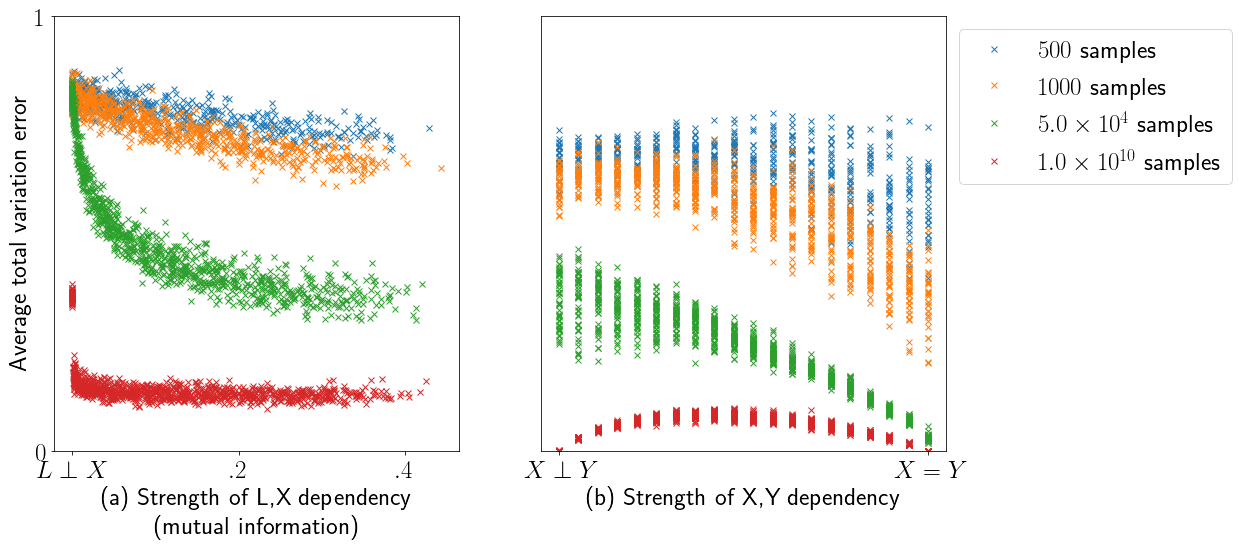
\includegraphics[width=.9\textwidth]{simident.png}\hfill{}

\hfill{}\begin{minipage}{.9\textwidth}
\caption{\textbf{Depending upon the exact model parameters, maximum likelihood estimation for $\beta$ may fail.}  We conducted a series of trials; in each trial we picked a sample size and ground-truth model parameters, simulated a dataset, calculated a maximum likelihood estimator for $\beta$, and compared it against the ground-truth.  Even when the sample size is effectively infinite, this estimator can fail.  Here we explore these failure modes.  To produce subfigure (a) each row of $\beta$ is drawn uniformly from the simplex; we explore how estimation error changes as we vary $\alpha$ to control the strength of the dependency between the variable $L$ and $X$.  When $L\perp X$, we see that maximum likelihood estimation fails significantly even with an essentially infinite number of samples.  To produce subfigure (b), we draw each row of $\alpha$ uniformly from the simplex and vary $\beta$ to control the dependency between $X$ and $Y$.  When $X\perp Y$ or $X=Y$ it is possible to get accurate estimates of $\beta$.  However, in a more typical case where the relationship between $X,Y$ is neither independent nor deterministic, we see that the maximum likelihood estimator fails to accurately determine $\beta$, even in the limit of essentially infinite data.  Both plots are consistent with Lemma \ref{lem:unident}, which states that there is no estimator for $\beta$ which will be consistent for every  ground-truth parameter. \label{fig:ident}}
\end{minipage}\hfill{}
\end{minipage}}\end{figure}

The previous section gives generic theoretical results about inference for the parameter $\beta$.  In this section we use simulations to get a more detailed understanding.

Our first simulations investigate Lemma \ref{lem:unident}, which states that there are cases where $N_L<N_X$ and $\beta$ cannot be identified even in the limit of infinite data.  We test this Lemma by exploring the performance of a maximum likelihood estimator for $\beta$ on different simulated datasets.  By varying the sample size and the ground-truth parameters of the model, we can explore this unidentifiability in detail:

\begin{itemize}
    \item Varying the sample size and the strength of the $L,X$ dependency.  Fix $N_X=N_Y=20$ and $N_L=15$.  We perform a series of trials.  In each trial we select $\pi$ and the rows of $\beta$ uniformly from the simplex.  The rows of $\alpha$ are chosen more carefully.  We will first generate $\tilde \alpha_1$ by sampling the rows uniformly from the simplex.  We then generate $\tau$ uniformly from the simplex and define $\tilde \alpha_2 = \mathbf{1}\tau^T$, i.e. every row of $\alpha_2$ is given by $\tau$.  Finally, we select $c\in[0,1]$ and define $\alpha=(1-c)(\tilde \alpha_1)+c\tilde \alpha_2$.  By varying $c$, we can control the mutual information between $L$ and $X$.  When $c=0$ the variable $L$ gives significant information about $X$; when $c=1$ we have that $L$ is independent of $X$.  Once $\pi,\alpha,\beta$ are selected, we select a sample size $n=m$, simulate a dataset, compute a maximum likelihood estimator $\hat \beta $ (see Appendix \ref{sec:mlmdetails} for our exact algorithm), and compute the average variation distance between $\beta$ and our estimate $\hat \beta$.  This average total variation distance is computed by averaging the row-by-row total variations between $\beta$ and  $\hat \beta$.  After performing a series of such trials, we visualize the results to obtain qualitative understanding of the performance of the maximum likelihood estimator $\hat \beta$.

    \item Varying the sample size and the strength of the $X,Y$ dependency.  Fix $N_X=N_Y=20$ and $N_L=15$.  We perform a series of trials.  For each trial, we select $\pi$ and the rows of $\alpha$ uniformly from the simplex.  To determine $\beta$, we first generate $\tau$ uniformly from the $N_Y$-simplex.  We then select $c\in[0,1]$ and define $\beta=c(\mathbf{1}\tau^T)+(1-c)I$.  By varying $c$, we can control the strength of dependency between $X$ and $Y$.  When $c=0$ we have that $X=Y$ (degenerate dependency); when $c=1$ we have that $X\perp Y$ (complete independence).  As above, for each trial we then compute a maximum likelihood estimator and compare the estimator to the ground-truth parameter.   
\end{itemize}

Figure \ref{fig:ident} shows the results.  We see that $\beta$ is much harder to estimate in some situations.  For example, the first simulation (Figure \ref{fig:ident}a) demonstrates that $\beta$ is harder to estimate when $L,X$ have low mutual information.  The second simulation (Figure \ref{fig:ident}b) shows a more complex picture; in some cases it is actually possible to get perfect estimation of $\beta$, even though $N_L<N_X$.  If $X,Y$ are independent or deterministically related, we see that perfect estimation becomes possible in the limit of infinite data.  However, in the more typical case where the relationship between $X$ and $Y$ neither independent nor deterministic, it appears that consistent estimation is not possible.   
 
We next investigate Theorem \ref{thm:consistency}, which implies that the Markov Link Intervals are asymptotically guaranteed to include the true parameter values for $\beta$.   Fix $N_X=N_Y=20$ and $N_L=15$.  We perform a series of trials.  In each trial we select $\pi$ and the rows of $\alpha,\beta$ uniformly from the simplex.  We then select a sample size $n=m$, simulate a dataset, and calculate the Markov Link Interval for the parameter $\beta_{1,1}$.  For each sample size $n$ we can plot a histogram of the differences between the upper bound $\hat \beta^{+}_{1,1}$ and the true parameter $\beta_{1,1}$.  A small positive value is ideal, indicating a tight bound on the true parameter.  Negative values are undesirable, since they indicate that the true parameter was in fact greater than the upper bound of the Markov Link Interval.  Large values are also undesirable since they indicate the bound was loose.  We can apply the same procedure to the differences between $\beta$ and $\hat \beta^{-}$.  By inspecting these histograms we obtian a qualitative sense for the performance of these intervals, complementing the theoretical guarantees of Theorem \ref{thm:consistency}.  The results are shown in Figure \ref{fig:simbound}.  We see that the true parameters are reliably bounded by the Markov Link Intervals, and these intervals shrink as we get more data.  However, even in the limit of essentially infinite data ($n=10^{10}$) we note that the width of the intervals does not vanish entirely.  This is consistent with the unidentifiability of $\beta$ demonstrated in Lemma \ref{lem:unident}.

These simulations are by no means exhaustive.  However, they yield a high-level overview of the estimation problem for this model.  First, estimation is easier when:
\begin{itemize}
    \item $L$ is highly informative about $X$.  
    \item $X,Y$ are either highly dependent or nearly independent
    \item Sample size is high
\end{itemize}
Second, even when estimation is difficult, the Markov Link Intervals give bounds which reliably contain the true parameter values.

\begin{figure}\fbox{\begin{minipage}{\textwidth}
% \begin{tabular}{cc}
% \includegraphics[width=.5\textwidth]{simIII.png} 
% & \includegraphics[width=.5\textwidth]{simII.png} \\
% %
% \begin{minipage}{.5\textwidth}(a) Performance depends on the $(L,X)$ dependency\end{minipage} 
% & \begin{minipage}{.5\textwidth}(a) Performance depends on the $(X,Y)$ dependency\end{minipage} 
% \end{tabular}
\hfill{}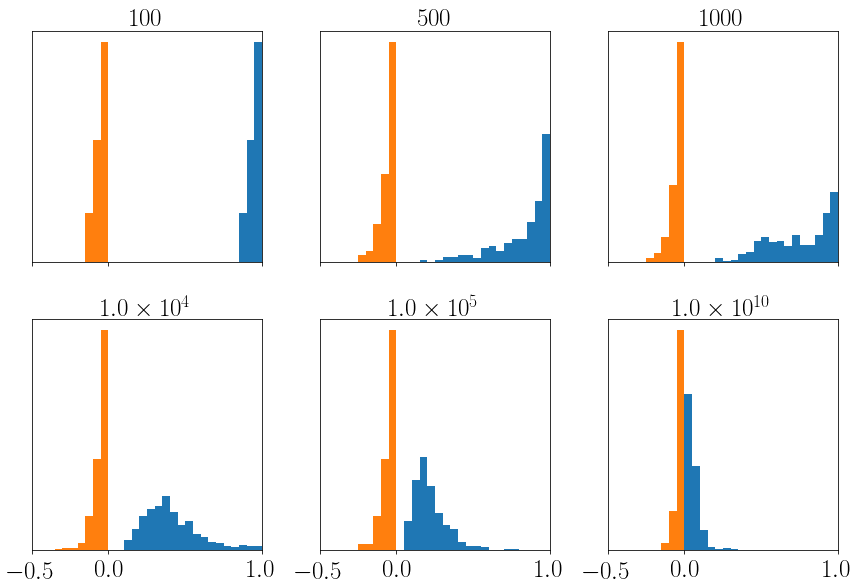
\includegraphics[width=.9\textwidth]{simbound.png}\hfill{}

\hfill{}\begin{minipage}{.9\textwidth}
\caption{\textbf{The Markov Link Intervals are conservative bounds around the true parameter estimates.}  We conducted a series of trials; in each trial we picked a sample size and ground-truth model parameters, simulated a dataset, calculated the Markov Link Intervals $\hat \beta^{-},\hat \beta^{+}$, and compared them against the truth.  For each trial we calculated both an upper slack ($\hat \beta^{+}-\beta$) and a lower slack ($\hat \beta^{-}-\beta$).   For each sample size $n \in \{100,500,1000,10^4,10^5,10^{10}\}$, we computed a histogram of all the upper and lower slack values in all of the simulations performed with that sample size.  We observe first that for every $n$ the upper slack is always positive and the lower slack is always negative, indicating the true value was contained inside our bound for every simulation.  Moreover, as the number of samples increases, we see that we can obtain tighter bounds; the magnitude of the upper and lower slacks decreases.  However, even in the limit of essentially infinite data ($n=10^{10}$) we note that the slack does not converge to zero.  This is consistent with the unidentifiability of $\beta$ demonstrated in Lemma \ref{lem:unident}. \label{fig:simbound}}
\end{minipage}\hfill{}
\end{minipage}}\end{figure}


%        _ _            
%   __ _| | | ___ _ __  
%  / _` | | |/ _ \ '_ \ 
% | (_| | | |  __/ | | |
%  \__,_|_|_|\___|_| |_|
                      


\section{Experiments for cell-types}
\label{sec:allen}

\begin{figure}\fbox{\begin{minipage}{\textwidth}
% \begin{tabular}{cc}
% \includegraphics[width=.5\textwidth]{simIII.png} 
% & \includegraphics[width=.5\textwidth]{simII.png} \\
% %
% \begin{minipage}{.5\textwidth}(a) Performance depends on the $(L,X)$ dependency\end{minipage} 
% & \begin{minipage}{.5\textwidth}(a) Performance depends on the $(X,Y)$ dependency\end{minipage} 
% \end{tabular}
\hfill{}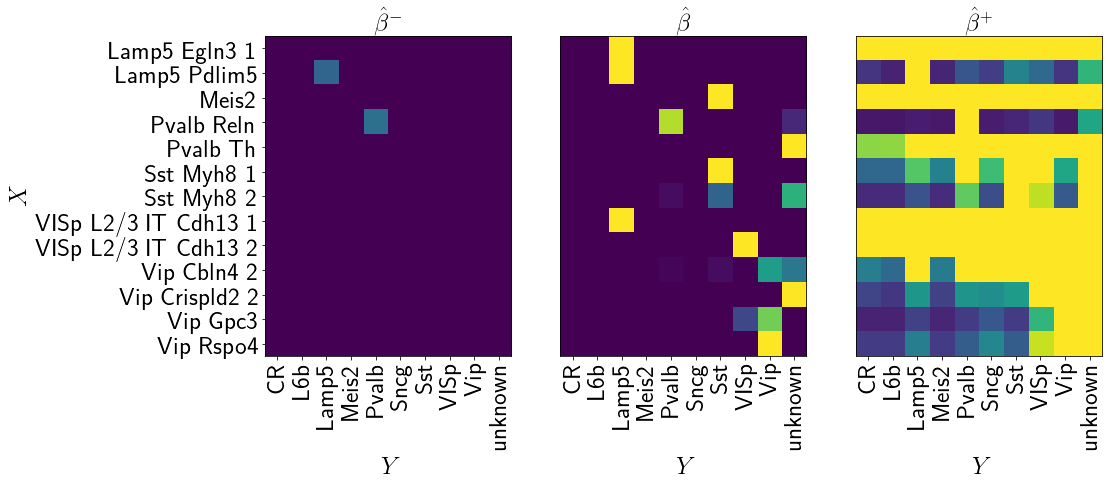
\includegraphics[width=.9\textwidth]{allen.png}\hfill{}

\hfill{}\begin{minipage}{.9\textwidth}
\caption{\textbf{Cell-type science.  Maximum likelihood estimation of $\beta$ suggests unlikely results about cell biology; Markov Link Intervals indicate plausible bounds.}  \label{fig:allen}
%
We performed unpaired measurement linkage for two ways of measuring the type of cells from mouse visual cortex.  The first method uses gene expression to obtain a definitive measurement of the cell-type, $X$.  The second method yields a considerably less reliable estimate for the cell-type, $Y$.  For each cell we also know the value of $L$, which corresponds to another noisy indicator about the cell-type $X$.  In one dataset we can observe $(L,X)$ for many cells; in another dataset we can observe $(L,Y)$ many other cells.  Using this data we construct three estimates for $\beta$, the matrix of parameters which defines the relationship between $X$ and $Y$.  For each possible index $(x,y)$, $\hat \beta^{-}_{x,y}$ estimates a lower-bound estimate for $\beta_{x,y}$, $\hat \beta_{x,y}$ is a maximum likelihood estimator, and $\hat \beta^{+}$ estimates an upper bound.  Due to identifiability issues $\hat \beta_{x,y}$ is not guaranteed to be consistent.  However, Theorem \ref{thm:consistency} shows that the Markov Link Interval $[\hat \beta^{-}_{x,y},\hat \beta^{+}_{x,y}]$ is asymptotically guaranteed to include the truth.  Above we show all three of these estimators for a selection of values of $(x,y)$; we visualize these values in a grid, where rows correspond to values of $x$, columns correspond to values of $y$, and the color of the square in the $(x,y)$ entry indicates the value of the corresponding parameter.  The values of $\hat \beta$ are nonsensical in many cases.  On the other hand, the Markov Link Interval suggests plausible bounds for the parameters and also indicates further experiments which would help refine these bounds.
}
\end{minipage}\hfill{}
\end{minipage}}\end{figure}

We now apply Markov Link Intervals to study the scientific problem which motivated their development.  

Every cell in a human body has the same DNA (to a first approximation), but some cells behave differently from others.  The biomolecular processes that drive this diversity are an area of active research \cite{wagner2018single,boudreau2018cell,he2018mechanical}.  Efforts such as the Human Cell Atlas project seek to map out a taxonomy of cell-types \cite{rozenblatt2017human}, thereby enabling a more systematic study of cellular diversity.  

At least at a coarse level, the cell-type $X$ of a given cell can be reliably determined by applying RNA sequencing techniques \cite{okaty2011cell}.  However, these techniques only measure one property of the cell: RNA expression. To determine the relationship between cell type and other properties of the cell, alternative techniques are required.  ``Patch-seq'' is one such approach \cite{cadwell2016electrophysiological}; this method obtains RNA, electrophysiological, and morphological properties at the single-cell level.  Unfortunately, the richness of the data comes at the cost of a degraded RNA signal, leading to a noisy estimate of the cell-type.  We will denote this noisy estimate as $Y$.  

For any cell it is thus impossible to measure a rich variety of cell properties \emph{and} reliably estimate the cell-type.  To understand the relationship between cell-type and these other cell properties, we therefore need some form of unpaired measurement linkage.  This linkage would allow us to determine the reliability of the noisy estimates $Y$, and thereby determine whether the relationship between cell-type and other cell properties can be reliably determined from the Patch-seq approach.  To facilitate this linkage, one can conduct experiments which make restrictions on which cells are are picked out, using a Cre/Lox system \cite{tasic2017shared}.  In each experiment, the probability that a particular cell will be picked out is entirely determined by the cell type $X$, and is thus statistically isolated from the noisy cell-type estimate $Y$.  By varying the experimental parameters we can change the distribution on which cells are picked out.  Letting $L$ denote these corresponding experimental parameters, we see that $L$ can act as a noisy independent indicator about the cell-type.  Markov Link Intervals should therefore give asymptotically consistent bounds on the reliability of the noisy estimate $Y$.  

The Allen Institute recently conducted a series of experiments using both traditional RNA sequencing as well as the Patch-seq technique \cite{tasic2017shared}.  The same Cre/Lox systems were used for both techniques.  For each sample in the traditional RNA sequencing dataset we observe both the cell-type ($X$) and the Cre/Lox indicator ($L$).  For each sample in the Patch-seq dataset we observe a both noisy estimate of the cell-type ($Y$) and the Cre/Lox indicator ($L$).  
% Note that the Patch cell-type estimates are only given at a coarse level of the taxonomy of cells.  For example, in the traditional RNA sequencing dataset a distinction is made between cell-type `Lamp5 Egln 1' and cell-type `Lamp5 Pdlim5,' whereas in the Patch-seq dataset we group all GABAergic neuronal cell-types characterized by high expression of `Lamp5' into a single coarse `cell class.'

We applied the Markov Link Intervals to the Allen Institute data try to determine the reliability of the noisy cell-type estimators $Y$ arising from Patch-seq approach.  We can visualize a maximum likelihood estimator as well as the Markov Link Intervals through heatmaps (see Figure \ref{fig:allen}).  We see that the maximum likelihood estimator sometimes gives nonsensical results.  For example, the maximum likelihood estimator suggests that a particular group of excitatory glutamatergic neurons from visual cortex are \emph{always} assigned to a GABAergic inhibitory type by the $Y$ variable.  This is quite unlikely, since even the noisy measurements of $Y$ can reliably determine between excitatory and inhibitory neurons \cite{cadwell2016electrophysiological,cadwell2017multimodal}. 

The Markov Link Intervals yield plausible bounds on the true model parameters.  For example, the lower bounds of the Markov Link Interval suggests that a sizable fraction of ``Lamp5 Pdlim5'' cells are indeed classified as ``Lamp5'' cells by the Patch method (note that the Patch method does not give fine-grained cell-type predictions, such as ``Lamp5 Pdlim5'', but instead only gives coarse class-level cell-type predictions, such as ``Lamp5'').  The upper bounds show that these cells are not commonly categorized into any group besides the `Lamp5' type and the the ``unknown'' type which the Patch method assigns to cells which it cannot identify.  Consider another example: for cells of type ``Sst Myh8-1'',  Markov Link Intervals give us considerably less certainty regarding the related type.  The intervals indicate that the Patch method does not typically classify these cells as ``CR,'' ``L6b,'' ``Meis2,'' ``Sncg,'' or ``Vip'' -- but it does not indicate how they are being classified.  At the extreme end, we have cells of type `Lamp5 Elgn3-1,' for which the Markov Link Intervals are completely vacuous.   It is possible that the Patch method perfectly classifies these ``Lamp5 Elgn3-1' cells; it is possible that it always misclassifies them; the available data cannot tell us either way.  

Parameters with large intervals suggest new experiments to perform in order to more closely determine the model parameters.  For example, the significant parameter ambiguity for cells with type ``Lamp5 Egln 1'' suggests we need a series of experiments with more distinct Cre/Lox experimental parameters that pick out cells of this kind.  If we could find a Cre/Lox procedure that obtained many ``Lamp5 Egln-1'' cells but no cells which Patch categorizes as ``Pvalb,'' this would show that ``Lamp5 Egln 1'' cells are not associated with Patch type `Pvalb.'  On the other hand, if we could find Cre/Lox parameters that select many `Lamp5 Egln 1' cells and also selects cells which are largely categorized as `Pvalb' by Patch, this would show the opposite.  If these additional experiments were performed, new Markov Link Intervals could be computed on the new data to determine what aspects of the link are still ambiguous.  

%                       _           _                 
%   ___ ___  _ __   ___| |_   _ ___(_) ___  _ __  ___ 
%  / __/ _ \| '_ \ / __| | | | / __| |/ _ \| '_ \/ __|
% | (_| (_) | | | | (__| | |_| \__ \ | (_) | | | \__ \
%  \___\___/|_| |_|\___|_|\__,_|___/_|\___/|_| |_|___/
                                                    

\section{Conclusions}

\label{sec:conclusions}

We here study ``unpaired measurement linkage,'' the problem of estimating a joint distribution $(X,Y)$ from two separate datasets, one with samples of $X$ and another with samples of $Y$.  Rigorous statistical analysis of this ill-posed problem are complicated by statistical error and identifiability issues.  Here we characterize both issues in the discrete settings when we can observe a third variable $L$ for each sample in both dataset, under the assumption that $L$ and $Y$ are independent conditioned in $X$.  

This assumption may hold under a variety of circumstances:

\begin{itemize}
    \item Quality control for manufacturing.   Consider a manufacturing process that produces components; to evaluate production quality, they use two different destructive tests.   The first kind of test is cheap, but its accuracy is unknown.  A more established test is accurate but expensive.  The manufacturer is interested in the link: given results from the cheap test ($X$), what might have been the results from the accurate test ($Y$)?   To estimate the link, we can uses different batches of production ($L$).  For example, $L$ might indicate the day on which a component was made.  The assumption: the link doesn't depend on the day the component was made. This is reasonable if the tests are performed on different days.  In this case, Markov Link Intervals can be used to calibrate the two kinds of tests.    

    \item Astronomy photography.  Consider an astronomer taking photographs of stars over time; depending on availability, some pictures are taken using one camera and other pictures are taken using a different camera.  To standardize the photos, the photographer is interested in the link: given a photo from one camera ($X$), what might the picture have looked like if it was taken with the other camera ($Y$)?  To estimate the link, the MLM uses different astronomical targets ($L$).   For example, $L$ might indicate which star is being photographed.  The assumption: the difference between the cameras is the same for each star.  This is reasonable as long as the camera settings are set to the same values for each star.  In this case, Markov Link Intervals can be used to standardize photographs from different cameras.  
 
    \item Personalized medicine.   Consider two sources of knowledge about how transcriptomes might help us personalize cancer medication.  We can measure the transcriptome of cancer cells from inside humans, but experimenting on humans is difficult and morally fraught.  We can also culture immortalized cells from human cancers and measure their transcriptomes;  experimenting on immortalized cells is cheap and straightforward.  To generalize work on immortalized cells to human patients, we need the link: given a cultured cell's transcriptome ($X$), what can we expect about the corresponding in-vivo transcriptome ($Y$)?  To estimate the link, we can use different types of cancer ($L$).  The assumption: the transcriptomic effects of culturing the cells is the same for each cancer type.  This may be reasonable as long as the cancer types are sufficiently similar.  In this case, the Markov Link Intervals  can be used to help generalize results from immortalized cells to real human patients.

    % \item Text/image correspondence.  Consider the problem of automatic captioning.  We can scrape images of people from the internet.  We can also find descriptions of people from literature.  Automatic captioning requires the link: given an image ($X$), what might its text description look like ($Y$)?  To estimate the link, the MLM can use different subject material ($L$).  For example, $L$ might indicate the climate of the location where the photograph was taken.  The assumption: the link is the same for people from different climates.  This is reasonable as long as the photograph itself indicates the important climate information, thereby creating an independence between $Y$ and $L$ after conditioning on $X$.    In this case, the MLM can be used to perform automatic captioning.

    \item Replication crisis and lab effects.  We would like to understand the differences in how two labs perform experiments.  These differences can be understood by looking at the link: given results from one lab ($X$), what results could we expect from another lab ($Y$)?  To estimate the link, we can use different specimen batches ($L$).  For example, $L$ might indicate a batch of mice, half of which were sent to one lab and half of which were sent to another lab.  The assumption: the lab effects are the same for each batch of mice.  
    % This is reasonable as long as the order in which the batches are processed is the same for both labs.  
    In this case, Markov Link Intervals can be used to discover ``lab effects'' that impede successful experimental replication.
\end{itemize}

When the conditional independence assumption holds, Markov Link Intervals  give provably consistent bounds on the joint distribution.  Simulations bear out the consistency of these bounds and also suggest estimation is easiest performs best when $L$ is predictive of $X$ and the relationship between $X$ and $Y$ is either deterministic or completely independent.  An application of the method to cell-type populations demonstrates the method's practical utility for unpaired measurement linkage problems.  One can imagine that these results could be extended to the continuous setting, though additional regularity conditions would be required.  

\bibliographystyle{unsrt}
\bibliography{refs}

%     _    ____  ____  _____ _   _ ____ _____  ___ 
%    / \  |  _ \|  _ \| ____| \ | |  _ \_ _\ \/ / |
%   / _ \ | |_) | |_) |  _| |  \| | | | | | \  /| |
%  / ___ \|  __/|  __/| |___| |\  | |_| | | /  \|_|
% /_/   \_\_|   |_|   |_____|_| \_|____/___/_/\_(_)
                                                 


\appendix

\section{Markov Link Interval details}
\label{sec:mlmdetails}

We here give a detailed explanation of how to compute the Markov Link Intervals from two unpaired datasets.

Let $n,m>0$ and $(L_1,X_1,Y_1),(L_2,X_2,Y_2) \cdots (L_{n+m},X_{n+m},Y_{n+m}) \sim p$, where $p(\ell,x,y)=\pi_\ell \alpha_{\ell,x} \beta_{x,y}$.  However, for $i\in 1\cdots n$ we cannot observe $Y_i$ and for $i\in n+1 \cdots n+m$ we cannot observe $X_i$.  Let $\LL(\theta)$ denote the likelihood of the observed data under the model under any particular choice of the parameters $\theta = \pi',\alpha',\beta'$.  Let $\LL^*$ denote the maximum value of $\LL$ over all possible parameters.  Define
\[
\hat \Theta=\left\{\theta:\ \LL(\theta) > \LL^* - \log(n + m)\right\}
\]
Our task is to calculate
\begin{align*}
[\hat \beta^-_{x,y},\hat \beta^+_{x,y}] &\triangleq \left[\min_{\pi',\alpha',\beta' \in \hat \Theta} \beta'_{x,y},\max_{\pi',\alpha',\beta' \in \hat \Theta}\beta'_{x,y}\right]
\end{align*}
Proceed as follows:

\begin{enumerate}
    \item Summarize the data into two matrices:
    \begin{align*}
    \DX_{\ell x} &= \#\{i\leq n: L_i=\ell,X_i=x\}\\
    \DY_{\ell y} &= \#\{i> n: L_i=\ell,Y_i=y\}
    \end{align*}

    \item Estimate the maximum likelihood.  The likelihood is given as
    \begin{align*}
    \LL(\pi,\alpha,\beta) = \sum_{\ell x} \DX_{\ell x} (\pi_\ell + \log \alpha_{\ell x}) + \sum_{\ell y} \DX_{\ell y} \left( \pi_\ell + \log \sum_x \alpha_{\ell x} \beta_{x,y}\right)
    \end{align*}
    We optimize this likelihood using Expectation Maximization.  Let
    \[
    \tau_{\ell x y} = \alpha_{\ell x}\beta_{x,y} / \sum_x \alpha_{\ell x'}\beta_{x',y}
    \]
    denote a posterior summary for the distribution of the unobserved values of the measurement $X$.  We then update the parameters by solving the surrogate problem
    \begin{align*}
    \max \left(\sum_{\ell x} \DX_{\ell x} (\pi_\ell + \log \alpha_{\ell x}) + \sum_{\ell y} \DX_{\ell y} \left( \tau_\ell + \sum_x \tau_{\ell x y}\log\alpha_{\ell x} \beta_{x,y}\right)\right)
    \end{align*}
    Note that this surrogate problem can be solved in closed form.  We proceed by iteratively updating our posterior summary then solving the the surrogate problem.  We terminate the algorithm when all parameters change less than $10^{-7}$ in a single iteration.

    \item Define 
    \begin{align*}
    \hat \Theta &= \left\{\theta:\ \LL(\theta) > \LL(\hat \theta) - \log(n+m)\right\}\\
    [\hat \beta^-_{x,y},\hat \beta^+_{x,y}] &\triangleq \left[\min_{\beta' \in \hat \Theta} \beta'_{x,y},\max_{\beta' \in \hat \Theta}\beta'_{x,y}\right]
    \end{align*}
    Let $x^*,y^*$ index a particular parameter for which we would like to compute $\hat \beta^-_{x^*,y^*},\hat \beta^+_{x^*,y^*}$.  We compute as follows:
    \begin{itemize}
        \item To compute $\min_{\beta' \in \hat \Theta} \beta'_{x^*,y^*}$.  The Lagrangian of this constrained problem may be written as
        \[
        V(\beta,\lambda) = \lambda \log \beta_{x^*,y^*} + L(\hat \alpha,\hat \beta)
        \]
        For any fixed $\lambda$, note that this problem has the same functional form as our original problem, and can be solved using the same algorithm as we used to find the maximium likelihood.  The updates for $\alpha$ are in fact identical.  The $\beta$ updates are only slightly different; combining the posterior summary and objective updates into one step, we obtain the updates
        \[
        \beta_{xy} \propto 
            \begin{cases} 
            {\beta}_{xy}\left(\frac{\lambda}{\beta_{xy}}  + \sum_{\ell}\alpha_{\ell x}\frac{\DX_{\ell y}}{\sum_{x}\alpha_{\ell x}{\beta}_{xy}}\right) & x=x^*,y=y^*\\
            {\beta}_{xy}\left(\sum_{\ell}\alpha_{\ell x}\frac{\DX_{\ell y}}{\sum_{x}\alpha_{\ell x}{\beta}_{xy}}\right) & \mathrm{otherwise}\\
            \end{cases}
        \]
        Let $\tilde \beta(\lambda,x^*,y^*)$ denote the optimizer of this inner problem.  To solve our overall problem, we need to find the correct value of $\lambda$, i.e. $\max \{\lambda:\ \tilde \beta(\lambda,x^*,y^*) \in \hat \Theta\}$.  We find this $\lambda$ using line-search.
        
        \item To compute $\min_{\beta' \in \hat \Theta^\epsilon} \beta'_{x^*,y^*}$.  This problem is equivalent to $\max_{\beta' \in \hat \Theta^\epsilon} \log \sum_{y\neq y^*} \beta'_{x^*,y}$.  This allows us to pose the problem just as we did above.  The resulting updates are given by:
        \[
        \beta_{xy} \propto 
            \begin{cases} 
            {\beta}_{xy}\left(\frac{\lambda}{\sum_{y'\neq y} \beta_{xy'}}  + \sum_{\ell}\alpha_{\ell x}\frac{\DX_{\ell y}}{\sum_{x}\alpha_{\ell x}{\beta}_{xy}}\right) & x=x^*,y\neq y^*\\
            {\beta}_{xy}\left(\sum_{\ell}\alpha_{\ell x}\frac{\DX_{\ell y}}{\sum_{x}\alpha_{\ell x}{\beta}_{xy}}\right) & \mathrm{otherwise}\\
            \end{cases}
        \]
    \end{itemize} 


\end{enumerate}

%                         __     
%  _ __  _ __ ___   ___  / _|___ 
% | '_ \| '__/ _ \ / _ \| |_/ __|
% | |_) | | | (_) | (_) |  _\__ \
% | .__/|_|  \___/ \___/|_| |___/
% |_|                            


\section{Proofs}
\label{sec:proofs}

\begin{lemma*}[Unidentifiability]  When $N_L<N_X$ there is no generally consistent estimator to infer $\beta$ from the data $(\DX,\DY)$. 
\end{lemma*}

\begin{proof}
    It suffices to show that there exist parameter choices $(\pi,\alpha,\beta)$ and $(\pi',\alpha',\beta')$ where $\beta\neq\beta'$ yet the distribution on $\DX,\DY$ remains the same.  In this case there would be not way to determine which of these parameter choices was correct, so no consistent estimator could be produced.  Note that the distribution on $\DX,\DY$ is entirely determined by $\pi$, $\alpha$, and $\gamma=\alpha\beta$.  Thus it suffices to find an example where $\alpha=\alpha',\beta\neq\beta',\alpha\beta=\alpha'\beta'$.  For a simple example, consider the case $N_L=1,N_X=N_Y=2$ with
    \[
    \alpha=\left(
        \begin{array}{cc}
        \frac{1}{4} & \frac{3}{4}\\
        \end{array}
    \right) \qquad
    \beta=\left(
        \begin{array}{cc}
        0.5 & 0.5\\
        0.1 & 0.9\\
        \end{array}
    \right) \qquad
    \beta'=\left(
        \begin{array}{cc}
        0.8 & 0.2\\
        0 & 1\\
        \end{array}
    \right) \qquad
    \]
\end{proof}

\begin{lemma*}[Discontinuity of observational equivalence classes]  Endow the space of observable distributions with the total variation metric.  Endow the space of sets of parameters $\pi,\alpha,\beta$ with the Pompeiu-Hausdorff metric.  The map from possible distributions on $\DX,\DY$ to observational equivalence classes of parameters is not continuous.   This mapping is sometimes discontinuous even around points where the rows of $\alpha$ are linearly independent and all parameters lie in the interior of the natural parameter space.  
\end{lemma*}

% sudo mount -v -t nfs4 -o nfsvers=4.1,rsize=1048576,wsize=1048576,hard,timeo=600,retrans=2 fs-d6b9599e.efs.us-east-1.amazonaws.com:/ groupstorage/

\begin{proof}
    We start by inspecting the two relevant spaces: the space of distributions on $\DX,\DY$ and the space of sets of parameters $\pi,\alpha,\beta$.
    \begin{itemize}
        \item The possible distributions on $\DX,\DY$.  Each distribution is parameterized by the triple $(\pi,\alpha,\beta)$, where $\pi$ lies in the probability simplex and $\alpha,\beta$ are right-stochastic matrices.  However, note that this parameterization is degenerate with respect to our chosen metric; any two points in this space, $(\pi,\alpha,\beta)$, $(\pi',\alpha',\beta')$, are considered equal as long as $\pi=\pi',\alpha=\alpha'$ and $\alpha\beta=\alpha'\beta'$.    In particular, the total variation distance between these two points is topologically equivalent to the $\mathscr{L}^1$ distance between for triples $(\pi,\alpha,\alpha \beta)$, $(\pi',\alpha',\alpha'\beta')$.  
        \item Sets of parameters.  Let $\Theta,\Theta'$ denote any two sets of parameters.  The Pompeiu-Hausdorff distance is the largest Euclidean distance from any point in either set to the closest point in the other set.
    \end{itemize}
    We are interested in the mapping from the first space to the second induced by observational equivalence classes, i.e.
    \[
    \pi,\alpha,\beta \mapsto \{(\pi,\alpha,\beta'):\ \alpha\beta=\alpha\beta'\}
    \]
    To show that this is discontinuous at some point $\pi,\alpha,\beta$ with respect to our chosen metrics, it suffices to find a sequence $\tilde \pi(\epsilon),\tilde \alpha(\epsilon),\tilde \beta(\epsilon)$ indexed by $\epsilon$ such that that 
    \begin{itemize}
        \item $\tilde \pi(\epsilon),\tilde \alpha(\epsilon),\tilde \alpha(\epsilon)\tilde\beta(\epsilon) \rightarrow \pi,\alpha,\alpha\beta$ in the $\mathscr{L}^1$ metric as $\epsilon\downarrow 0$
        \item $\Theta(\epsilon)\triangleq \{(\pi(\epsilon),\alpha(\epsilon),\beta'):\ \alpha(\epsilon)'\beta'=\gamma\}$ fails to converge to $\Theta(0)\triangleq \{(\pi,\alpha,\beta):\ \alpha\beta'=\gamma\}$ in the Pompeiu-Hausdorff metric.
    \end{itemize}
    We exhibit such a case.  Fix any $\pi$ strictly on the interior of the simplex.  Let $\Theta(0)=\{(\pi,\alpha,\beta'):\ \alpha\beta'=\alpha\beta\}$, where
    \[
    \alpha=\left(\begin{array}{ccc}
    \frac{1}{2} & \frac{1}{4} & \frac{1}{4}\\
    \frac{1}{3} & \frac{1}{3} & \frac{1}{3}
    \end{array}\right)
    \qquad
    \beta=\left(\begin{array}{cc}
    0 & 1\\
    \frac{1}{2} & \frac{1}{2}\\
    \frac{1}{2} & \frac{1}{2}
    \end{array}\right)
    \qquad
    \alpha\beta=\left(\begin{array}{cc}
    \frac{1}{4} & \frac{3}{4}\\
    \frac{1}{3} & \frac{2}{3}
    \end{array}\right)
    \]
    For each $\epsilon>0$ let $\Theta(\epsilon) =\{(\pi,\tilde \alpha(\epsilon),\beta'):\ \tilde \alpha(\epsilon)\beta'=\tilde \alpha(\epsilon) \tilde \beta\}$, where
    \[
    \tilde \alpha(\epsilon)=\left(\begin{array}{ccc}
    \frac{1}{2} & \frac{1}{4}-\frac{\epsilon}{2} & \frac{1}{4}+\frac{\epsilon}{2}\\
    \frac{1}{3} & \frac{1}{3}-\frac{\epsilon}{3} & \frac{1}{3}+\frac{\epsilon}{3}
    \end{array}\right)\qquad
    \tilde \beta=\left(\begin{array}{cc}
    0 & 1\\
    1 & 0\\
    0 & 1
    \end{array}\right)\qquad
    \tilde \alpha(\epsilon) \tilde \beta=\left(\begin{array}{cc}
    \frac{1}{4} -\frac{\epsilon}{2}& \frac{3}{4}+\frac{\epsilon}{2}\\
    \frac{1}{3}-\frac{\epsilon}{3} & \frac{2}{3}+\frac{\epsilon}{2}
    \end{array}\right)
    \]
    Now observe:
    \begin{itemize}
        \item $\pi,\tilde \alpha(\epsilon),\tilde \alpha(\epsilon)\beta \rightarrow \pi,\alpha,\alpha\beta$ in $\mathscr{L}^1$ metric as $\epsilon\downarrow 0$
        \item $\Theta(\epsilon)$ fails to converge to $\Theta(0)$.  Indeed consider any $\beta' \in S(\epsilon)$.  Algebraic manipulations yield that $\beta_{11}'=2(\beta_{21}'-1)\epsilon$ for every $\beta' \in S(\epsilon)$.  This is a negative value unless $\beta_{21}\geq 1$, ergo $\beta' \in S(\epsilon)$ is only a valid right-stochastic matrix if $\beta_{21}'=1$.  On the other hand, $\beta \in S(0)$ satisfies $\beta_{21}=1/2$.  It follows that the Pompeiu-Hausdorff from $\Theta(0)$ to $\Theta(\epsilon)$ is at least $1/2$ for every $\epsilon>0$.
    \end{itemize}

    This shows that the mapping is discontinuous at $\pi,\alpha,\beta$.  Furthermore note that the rows of $\alpha$ are linearly indendent.  Moreover, $\pi$ lies strictly on the interior of the simplex, as does every row of $\alpha$ and $\alpha\beta$.  Thus the distribution corresponding to $\pi,\alpha,\beta$ lies strictly on the interior of the natural parameter space.
\end{proof}

\begin{thm*}[Consistency for positive $\beta$]  Let the rows of $\alpha$ be linearly independent and let $\beta_{x,y}\geq c>0$.  Define $\gamma$ as the $N_L\times N_Y$ right-stochastic matrix
\[
\gamma_{\ell y} \triangleq \sum_{x} \alpha_{_\ell x} \beta_{x,y}
\]
Let $\hat \pi, \hat \alpha, \hat \gamma$ denote any consistent estimators for $\pi,\alpha,\gamma$.  Consider $\{\beta':\ \hat \alpha\beta'=\hat \gamma \}$, the equivalence class for the observations $\DY$ after fixing the estimate $\hat \alpha$.  The distance between the point $\beta$ and this set converges to zero in probability.  
\end{thm*}

\begin{proof}
Fix any $\alpha,\beta$.  It suffices to show that by ensuring $\left|\alpha'-\alpha\right|<\delta,\left|\gamma'-\alpha \beta\right|<\delta$ for $\delta$ sufficiently small we can ensure that $\beta$ is arbitrarily close to some valid right-stochastic matrix in the set $\{\beta':\ \alpha'\beta' = \gamma'\}$.  Let $\tilde{\beta}$ denote the orthogonal projection of $\beta$ to this set.  Note that since the rows of $\alpha$ are independent we can ensure the rows of $\alpha'$ are also independent by taking $\delta$ sufficiently small.  In particular, we can bound the spectral norm of the pseudoinverse of $\alpha'$, and thereby ensure that $\left|\tilde{\beta}_{x,y}-\beta_{x,y}\right|<\epsilon$ for every $x,y$ by taking $\delta$ sufficiently small. Finally, the positivity of $\beta$ allows to ensure that $\tilde \beta$ is a valid right-stochastic matrix.  Thus $\tilde \beta$ is indeed a point in the observational equivalence class which is arbitrarily close to $\beta$.  
\end{proof}

\begin{thm*}[Consistency of $\hat \Theta$] Let $n,m\rightarrow\infty$ such that $|\log(n/m)|<M$.  Then:
\begin{enumerate}
    \item $\hat \Theta$ is asymptotically guaranteed to contain the true parameter values.  
    \item $\hat \Theta$ concentrates for $\pi,\alpha,\alpha\beta$. Let $\xi(\pi',\alpha',\beta')$ denote the maximum of the Euclidean differences $|\pi-\pi'|$, $|\alpha-\alpha'|$, $|\alpha\beta-\alpha'\beta'|$.  Then $\max_{\theta \in \hat \Theta} \xi(\theta)$ converges to zero in probability.   
\end{enumerate}
\end{thm*}
\begin{proof} A corollary of Lemma \ref{lem:sqrtset}, below.  A minor correction is necessary to deal with the fact that we have two sets of independent samples instead of a single list of independent samples.  Fix any $n'>0,m'>0$.  Arrange the $\DX,\DY$ into $T$ independent groups of samples, each containing $n'>0$ samples from $\DX$ and $m'>0$ samples from $\DY$.  Drop samples at the end that cannot be fit into even groups.  Since we have required $|\log(n/m)|<M$, note that can obtain an arbitrarily large number of such groups in the limit.  We can now understand our data as a list of $T$ independent samples drawn from a distribution $p^\Pi$.  Here 
\[
p^\Pi(\ell_1,x_1\cdots \ell_{n'},x_{n'},\ell_{n'+1},y_{n'+1}\cdots \ell_{n'+m'},y_{n'+m'})
\]
is defined as the product of the corresponding distributions arising from $p$.

Now apply Lemma \ref{lem:sqrtset} to this grouped data in the limit as $T\rightarrow \infty$, where the set $S$ indicates the image of our parameterization of $p$. The lemma shows that the true parameter $\pi,\alpha,\beta$ is asymptotically guaranteed to lie in the set $\hat \Theta$; this proves the first claim of our theorem.  Second, the theorem shows that $\pi',\alpha',\beta'$ will be asymptotically excluded as long as $p^\Pi(\cdot; \pi',\alpha',\beta') \neq p^\Pi(\cdot; \pi,\alpha,\beta)$.  Observe that $p^\Pi(\cdot; \pi',\alpha',\beta') \neq p^\Pi(\cdot; \pi,\alpha,\beta)$ if and only if $\pi',\alpha',\beta'$ lies in the true observational equivalence class, i.e. $\pi=\pi',\alpha=\alpha',\alpha\beta=\alpha'\beta'$. Thus any set of parameters whose Kullback-Leibler divergence from the truth is bounded away from zero will asymptotically fail to intersect $\hat \Theta$.  To conclude our proof of the second claim, note that Pinsker's inequality lower-bounds this divergence by the Euclidean distance on the space of the observable distributions $\pi,\alpha,\alpha\beta$.
\end{proof}

\begin{lemma}  \label{lem:sqrtset} Let $(W_1 \cdots W_n)\ \mathrm{i.i.d} \sim p^*$, where $p^*$ is a probability mass function on a finite number of atoms.  Let $\LL(p)=\log\sum_i \log p_{W_i}$ denote the log likelihood for any $p$ on the simplex.  Let $S$ denote any subset of the simplex with $p^* \subset S$.  Let $\hat p = \arg \max_{p \in S} \LL(p)$ denote a maximum likelihood estimator.  Fix any $\delta>0$ and define 
\[
\hat \Theta = \{\theta :\ \LL(\theta) > \LL(\hat \theta) - \delta \log n\}
\]
Then:
\begin{enumerate}
    \item The probability that $p^* \in \hat \Theta$ is asymptotically unity.
    \item Let $D(p^*||p)$ denote the Kullback-Leibler divergence from $p^*$ to $p$ for any $p$ on the simplex.  Let $\Gamma(\epsilon)= \{p:\ D(p^*||p)>\epsilon\}$.  The probability that $\Gamma(\epsilon)$ and $\hat \Theta$ intersect asymptotically vanishes for any $\epsilon>0$.
\end{enumerate}
\end{lemma}
\begin{proof}  The proof is straightforward because we have required $p$ is a probability mass function with a finite number of atoms.  
\begin{enumerate}
    \item $p^* \in \hat \Theta$ with high probability. Since $\log n\rightarrow \infty$ it suffices to show that $\limsup_{n\rightarrow\infty} \mathbb{E}[\LL(\hat p)- \LL(p^*)]$ is bounded.  The only slight subtlety here is that the estimator $\hat p$ is required to lie in the arbitrary set $S$ -- otherwise the usual asymptotic theory would immediately give that $\LL(\hat p)- \LL(p^*)$ is asymptotically $\chi^2$ with $\#\{x:\ p(x;p^*)>0\}-1$ degrees of freedom.  However, since $\hat p$ arises from optimizing over a \emph{restricted} domain, it follows that $\LL(\hat p)- \LL(p^*)$ is actually stochastically dominated by this same $\chi^2$ distribution.  Thus the expectation in question is bounded.
    
    \item Incorrect parameters are excluded.  First observe that the result holds pointwise, i.e. for any $\epsilon>0,p \in \Gamma(\epsilon)$ we have that $p$ is asymptotically excluded from $\hat \Theta$.  To see this, observe that the central limit theorem yields, asymptotically, that
    \[
    V(p) \triangleq \frac{1}{\sqrt{n}} (\LL(p^*) - \LL(p) - nD(p^*||p)) \sim \mathcal N\left(0,\sigma^2_p\right)
    \]
    where $\sigma^2_p$ is the variance of the corresponding single-sample estimator for the KL divergence.   Thus   
    \begin{align*}
    \mathbb{P}\left(p \in \hat \Theta\right) 
        &=\mathbb{P}\left((\LL(\hat p) - \LL(p^*))+ (\LL(p^*) - \LL(p) -nD(p^*||p)) < \delta \log n - nD(p^*||p)\right)\\ 
        &=\mathbb{P}\left(V(p) < \delta \frac{\log n}{\sqrt n} - \sqrt{n}D(p^*||p) - (\LL(\hat p) - \LL(p^*))/\sqrt{n}\right) 
    \end{align*}
    This probability vanishes whenever $D(p^*||p)>0$, since the right-hand-side of the inequality inside the probability expression escapes to $-\infty$.  Thus every $p \in \Gamma$ is eventually excluded from $\hat \Theta$.  To conclude our proof of the second claim, note that $\hat \Theta$ is a convex set whose eccentricity is bounded by the ratio between the lowest and highest nonzero value in the empirical distribution of the $X$s; since there are a finite number of atoms this eccentricity is thus asymptotically bounded.  Moreover, note that $p \mapsto D(p^*||p)$ is convex and uniformly continuous in neighborhoods of $p^*$.   We can therefore find a grid of points $p\in \Gamma(\epsilon/2)$ whose convex hull contains $p^*$, such that any convex set which does not intersect those points must lie in the complement of $\Gamma(\epsilon)$.  By applying the pointwise result to this finite collection of points, we obtain our uniform result.

\end{enumerate}
\end{proof}

\end{document}